\appendix
\chapter{Jelmagyarázat} \label{legend}
\begin{description}
\item[$P$]  a termékek halmaza
\item[$b_p$]  a legyártott batch-ek darabszáma az adott konfigurációban
\item[$s_p$]  a termék batch mérete (fix batch méret esetén) [Kg]
\item[$s_p^{min},s_p^{max}$]  adott termékhez tartozó lehetséges legkisebb, legnagyobb batch méret (válzotó batch méret esetén) [Kg]
\item[$S$]  a forgatókönyvek halmaza
\item[$prob_s$]  s forgatókönyv valószínűsége $s	\in S$
\item[$dem_{s,p}$]  p termék iránti kereslet az s forgatókönyvben $s	\in S, p	\in P$ [Kg]
\item[$price_{s,p}$]  p termék ára az s forgatókönyvben $s	\in S, p	\in P$ [Cost Unit/Kg]
\item[$oc_{s,p}, uc_{s,p}$]  p termék túl-, és alul termelési költsége s forgatókönyvben $s	\in S, p	\in P$ [Cost Unit/Kg]
\item[$ExpProfit_p(x)=\sum_{s \in S}prob_s \cdot profit_{s,p}(x)$]  $p$ termék $x$ értékben vett várható profit értéke
\end {description}
\begin{equation*}
Profit_{s,p}(x)= \begin{cases}
            price_{s,p}\cdot x-(dem_{s,p}-x) \cdot uc_{s,p}\qquad \text{ha } x<dem_{s,p} \\
            price_{s,p} \cdot dem_{s,p}-(x-dem_{s,p}) \cdot oc_{s,p}\qquad \text{egyébként}
       \end{cases}
\end{equation*}

\chapter{Input fájlok} \label{input_files}
\begin{figure}[H]
\begin{center}
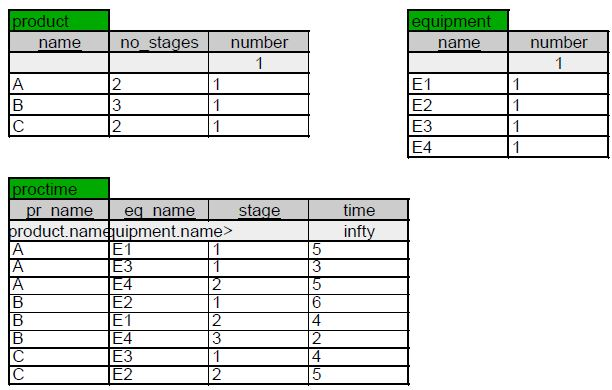
\includegraphics[scale=0.4]{multipurposeOds}
\caption{A \textit{multipurpose.ods} fájl}
\label{multipurpose_ods}
\end{center}
\end{figure}
\begin{figure}[H]
\begin{center}
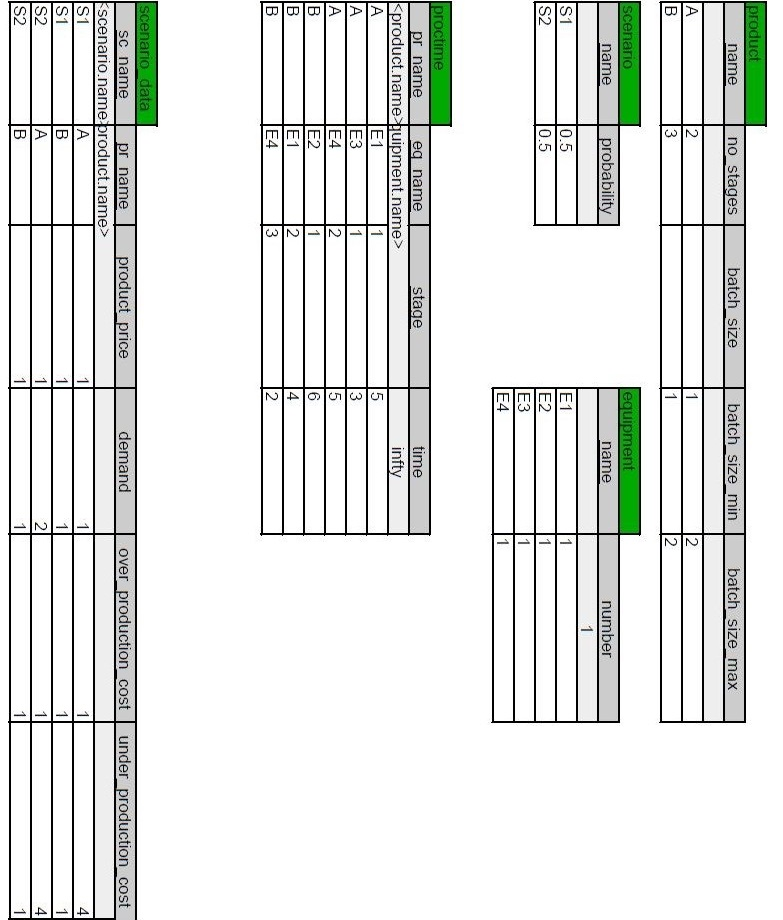
\includegraphics[scale=0.5]{stochasticOds}
\caption{A \textit{stochastic.ods} fájl}
\label{stochastic_ods}
\end{center}
\end{figure}
\begin{figure}[H]
\begin{center}
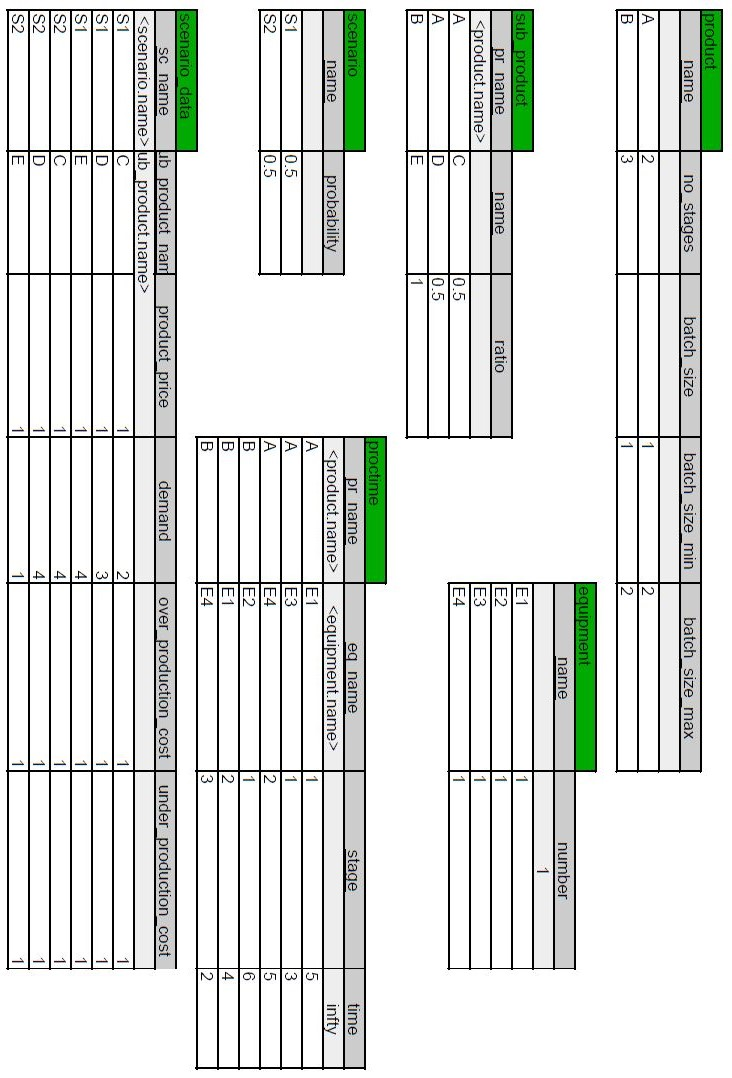
\includegraphics[scale=0.5]{stochasticExtendedOds}
\caption{A \textit{stochastic\_extended.ods} fájl}
\label{stochastic_extended_ods}
\end{center}
\end{figure}
\chapter{CD melléklet tartalma} \label{cd}
\dirtree{%
.1 CD melléklet/.
.2 Algoritmusok.
.3 DO\_Sgraph\_Makespan\_Minimization.odg.
.3 DO\_Sgraph\_Throughput\_Maximization.odp.
.2 Tesztelés.
.3 Teszteredmények.
.4 DeterministicTestResults.ods.
.4 StochasticTestResults.ods.
.4 StochasticMultiproductTestResults.ods.
.3 Tesztfájlok.
.4 Determinisztikus.
.4 Sztochasztikus.
.4 Sztochasztikus\_Multiproduct.
.2 Solver kód.
.3 README.md.
.3 input.
.4 multipurpose.ods.
.4 stochastic.ods.
.4 stochastic\_extended.ods.
.3 src.
.4 arguments.cpp.
.4 base.
.5 piecewiselinearfunction.h.
.5 piecewiselinearfunction.cpp.
.4 lib.
.5 relationalproblemreader.h.
.5 relationalproblemreader.cpp.
.4 solver.
.5 mainsolver.cpp.
.5 recipe.h.
.5 recipe.cpp.
.5 sgraph.h.
.5 sgraph.cpp.
.5 statistics.h.
.5 throughputsolver.h.
.5 throughputsolver.cpp.
.5 throughputui.cpp.
}